Figure 1 presents the generic pipeline, divided into two main parts: data preparation for ASR and separately for AST. To provide a better understanding of each step, its content, and the underlying experiments, we will discuss them in detail in the following subsections.

\subsection{ASR Data Pipeline}

Building on prior research \cite{mosel}, we identified Whisper-large-v3 \cite{radford2023robust} as a strong candidate for pseudo-labeling due to its robust performance, multilingual capabilities, and open license. However, its direct application requires careful adjustments and filtering due to several challenges. Whisper exhibits reduced accuracy in low-resource languages and is prone to hallucinations, particularly in its turbo variant. It struggles with noise and non-speech segments, necessitating a robust voice activity detection (VAD) system. Additionally, language identification errors, fixed 30-second segment requirements, and lack of case control in output text further complicate its use. 
Addressing these limitations is crucial for effectively leveraging Whisper for pseudo-labeling leading us to design Granary pipeline which we will outline in this section.

All files were converted to FLAC or WAV formats at a sample rate of 16 kHz and mono-channel to ensure consistency. Additionally, we set a maximum duration of 40 seconds for the final audio files\cite{koluguri2024longer}. 





\subsubsection{Long-form Audio Segmentation}
\label{subsec:long-form-segmentation}

The availability of ground truth transcriptions in the YouTube data necessitated the use of an alignment algorithm to segment the audio and assign the corresponding transcriptions to each segment. We experimented with multiple alignment methods, including VAD, NeMo Forced Alignment (NFA)\cite{rastorgueva2023nemo}, Time-Duration-Transducer (TDT)\cite{koluguri2024longer} decoder and Whisper timestamps.

Using ASR models (Parakeet\cite{rekesh2023fast} \& Whisper) for timestamp generation, we compared ground truth and intermediate transcripts, finding that pseudo-labels consistently improved segmentation results. Thus, we adopted them for data processing in the Granary corpus (evaluation results omitted for space constraints). When evaluating segmentation methods, we found no significant differences in final model performance. Therefore, we chose Whisper model timestamps for the YODAS and YTC sets and Parakeet\footnote{\url{https://hf.co/nvidia/parakeet-tdt_ctc-110m}} model timestamps for the LibriLight dataset. Further analysis showed that Whisper's segment-level timestamps were poor at word alignment but effective for speech/non-speech detection. This led us to run a second-pass inference with Whisper to generate transcripts for newly segmented audio. In contrast, TDT Decoder timestamps provided high-quality segment-level alignment, eliminating the need for a second inference pass for approximately 60k hours of En data.


\begin{figure}[htbp]
    \centering
    \caption{Example of MOSEL Transcription Truncation Issue and the same sentence transcription with Granary Pipeline.}
    \begin{tcolorbox}[
        colframe=black,
        colback=white,
        arc=2mm,
        width=\linewidth,
        boxrule=0.2mm,
    ]
    \textbf{MOSEL Transcription:}  

    a Council recommendation on the strengthening cooperation against vaccine-preventable diseases. Thank you very much for your attention. \textcolor{red}{{[MISSING PART]}}

    \vspace{0.5em}
    \textbf{Granary Transcription:}  

    a Council recommendation on the strengthening cooperation against vaccine-preventable diseases. Thank you very much for your attention. \textcolor[rgb]{0,0.5,0}{{And thank you very much, Madam. Colleagues, our debate is closed.}}
    \end{tcolorbox}
    \label{fig:mosel_transcription}
\end{figure}

\subsubsection{Two-Pass Inference}

Building on the previous subsection, where we highlighted the need for generating a high volume of pseudo-labels—even for ground truth samples—we initiated the Whisper-large-V3 pipeline using FasterWhisper\cite{faster-whisper} with a beam size of 5 and a chunk batch of 16. Following MOSEL's best practices \cite{mosel}, we performed two-pass inference: first for language ID prediction, then for transcription, using the predicted language ID as metadata to improve data quality. We also integrated Silero VAD \cite{silerovad} into the pipeline, which, with 400ms padding, minimized truncated transcriptions (as presented in Figure \ref{fig:mosel_transcription}) and reduced hallucinations by focusing inference on detected speech regions. Additionally, we modified the FasterWhisper source code to extract language IDs for each segment, enhancing our filtration pipeline.


\subsubsection{LID Verification}
We also noticed that eliminating data points where Whisper's predicted LID does not align with the target language significantly enhances the performance of the speech recognition model. 
% We applied this insight by conducting Language ID verification across all our subsets. 
We filtered out samples with multiple languages, common in the Voxpopuli dataset due to interpreter voices. For Granary's Voxpopuli set, we further refined filtering by excluding samples with low confidence Language ID predictions  ($\texttt{lid\_prob} < 0.8$).



\subsubsection{Robust Data Filtration}

Significant portion of filtration occurs at this stage of our pipeline, which involves three primary metrics for conducting the filtration process. First, we eliminate instances where any of the three hallucination flags are active, signaling the presence of \textit{i)} repeated \textit{n}-grams, \textit{ii)} long words, or \textit{iii)} frequently hallucinated phrases. The latter is particularly noteworthy; leveraging custom modifications to Whisper-large-V3 and V3-turbo, we compiled language-specific lists of commonly hallucinated phrases. These include both specific terms, such as \textit{"Sous-titrage Société Radio-Canada"} in French, and broadly used expressions like \textit{"Thank you very much"}. We use these lists to detect and filter hallucinated audio samples, and they will be made available as part of our open-source pipeline.

Character rate filtering is another crucial step. Using language- and corpus-specific heuristics, we eliminate speech-transcription pairs with anomalously low or high character rates, assuming such samples may contain non-speech segments, poor pseudo-labels, or unusual speech patterns.

Finally, we apply character set filtering by excluding any character deemed "invalid" for the Granary corpus. This comprehensive superset of over 300 characters and symbols ensures coverage of the alphabets across all 25 represented European languages.


\subsubsection{LLM-Powered P\&C Restoration}

The Granary corpus relies on pseudo-labeled data from Whisper, necessitating steps to enhance quality and reduce dependence on Whisper's performance. To address this, we applied punctuation and capitalization restoration using the large language model Qwen 2.5-7B-Instruct.

We crafted a language-specific prompt directing the model to assess and correct punctuation and capitalization, supplemented by multiple correction examples. To maintain output quality, we implemented character set filtering and Qwen hallucination filtering. A heuristic was used: if Qwen's output deviated from Whisper's transcriptions by more than a 5\% character error rate, the original pseudo-labels were retained. This margin allows Qwen to potentially correct typos or refine formulations. However, the quality of these modifications remains a subject for further testing.


\begin{figure*}[ht]
    \centering
    \caption{Total hours per language per task (ASR and AST) in Granary after final filtering (log scale). English has the most hours (275k for ASR), while Ukrainian has the least (932.67 for ASR, 608.80 for X$\rightarrow$En).}
    % \includesvg[width=1\linewidth]{figures/hrs_chart.svg}
    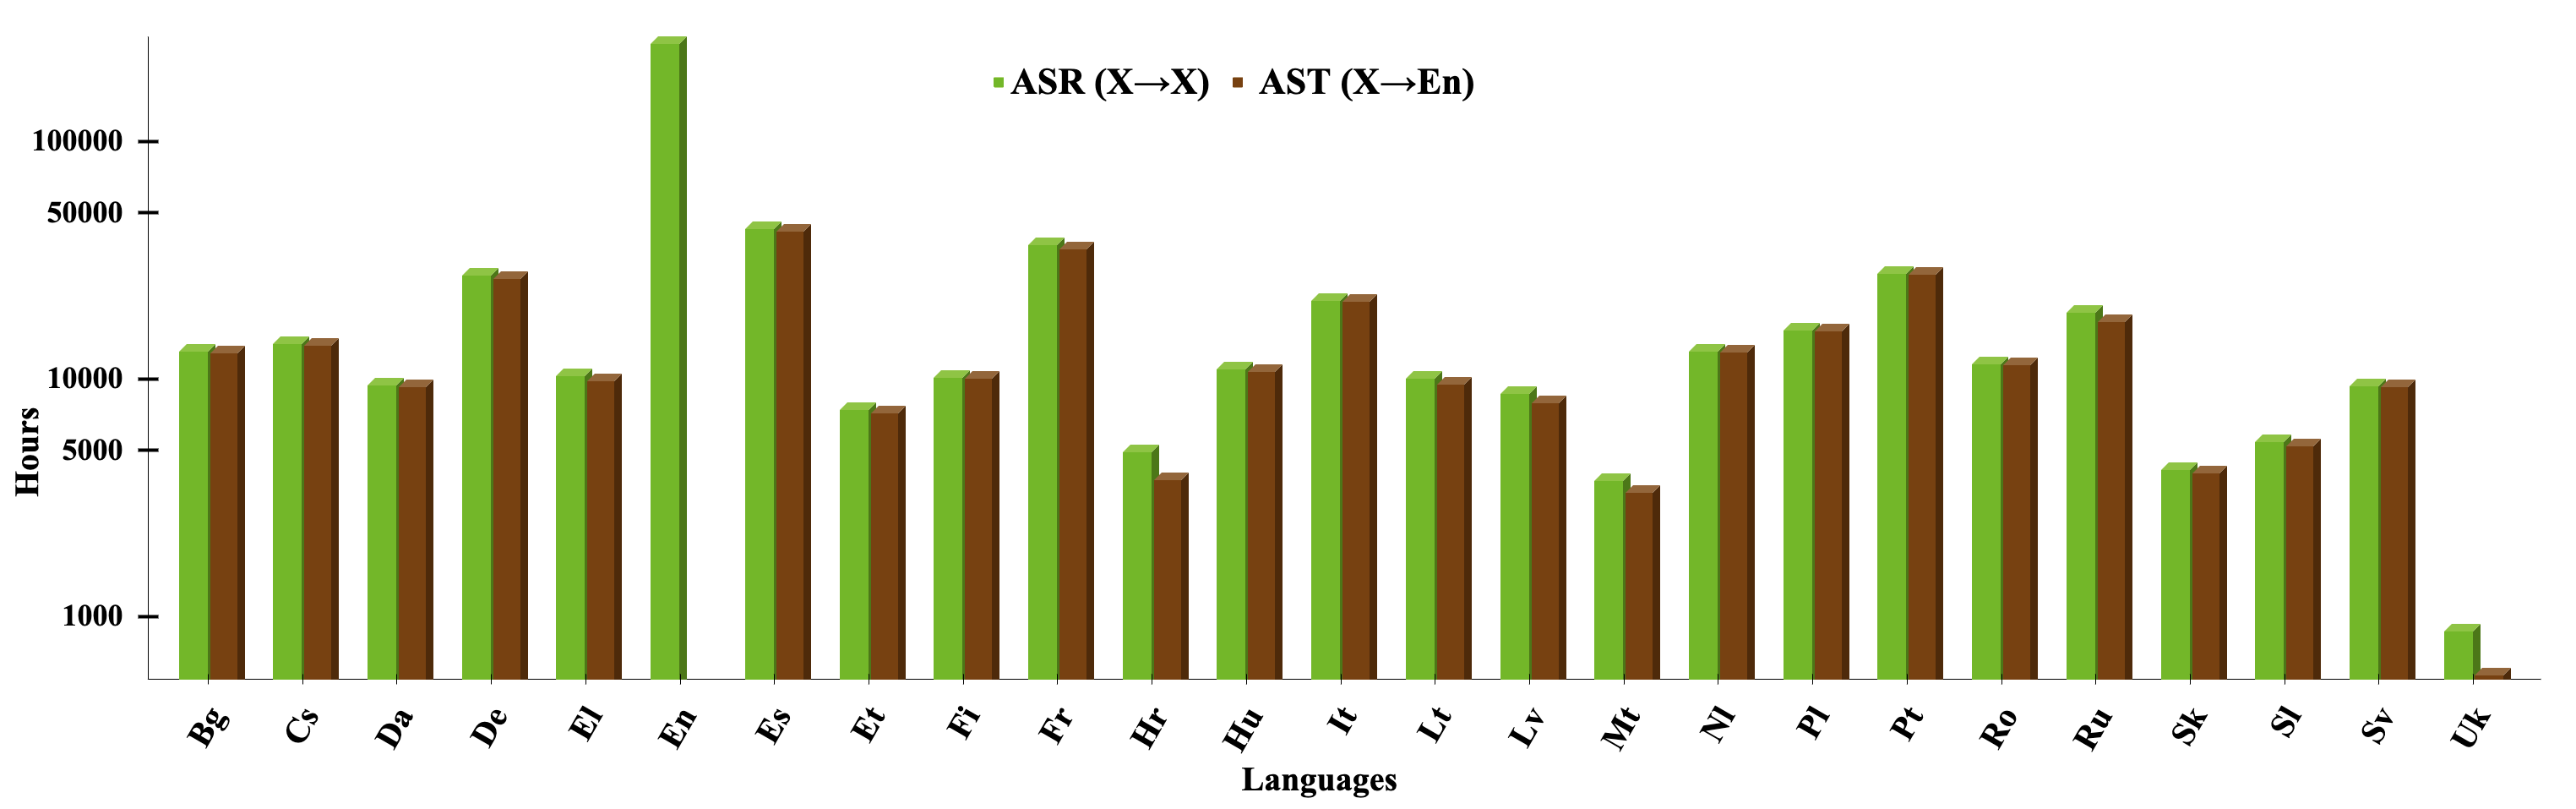
\includegraphics[width=1\linewidth]{figures/hrs_chart.png}
    \label{fig:filtered_hrs_chart}
\end{figure*}

\subsection{AST Data Pipeline}

\subsubsection{Selection of Pseudo-Labeling Models}

We benchmarked several translation models to select the best model for X$\rightarrow$En AST pseudo labeling.
Our candidate models include LLMs such as Alma-13B-R \cite{xu2024a}, Qwen-2.5-7B \cite{qwen2}, EuroLLM-1.7B, and EuroLLM-9B \cite{DBLP:journals/corr/abs-2409-16235}, as well as encoder-decoder models such as 
Riva-Megatron Any2Any model\footnote{\url{https://catalog.ngc.nvidia.com/orgs/nvidia/teams/riva/models/riva_megatronnmt_any_any_1b}}. 
We excluded API-only models such as GPT-4o out of cost concerns, as well as TowerInstruct-13B and Aya-23 models because of non-commercial licenses.
Alma-13B-R and Qwen-2.5-7B were excluded during preliminary study, because the former under-performs significantly in speech domain (despite achieving impressive results on WMT test sets), and the latter suffers from hallucination issues during pseudo-labeling.
After a final comparison on the Flores dataset \cite{goyal-etal-2022-flores} covering all 24 translation directions of interest, we identified EuroLLM-9B as the best-performing model for AST data synthesis.

\subsubsection{LLM Inference}

We perform LLM inference on processed ASR data using the translation prompt from EuroLLM's model card.
For optimal speed, we use greedy inference with vLLM.
We also experimented with beam search, which provided a slight improvement for EuroLLM-1.7B but had diminishing returns for the 9B model, making the added computational cost unjustifiable.

\subsubsection{Filtration}

Prior work \cite{koehn-etal-2020-findings,peter-etal-2023-theres,finkelstein-etal-2024-introducing} has emphasized the importance of training data filtration for optimal translation performance.
Although our pseudo-labeled data is generated using an LLM optimized for translation, a small but persistent fraction of hallucinated examples remains.
This motivates us to develop an efficient and effective data filtration pipeline for our synthetic AST data.

Our data filtration pipeline is implemented in 
NeMo-Curator\footnote{\url{https://github.com/NVIDIA/NeMo-Curator/}},
a GPU-accelerated data curation toolkit.
Our filtration steps include a re-implementation of the length ratio filtering step from Moses
\footnote{\href{https://github.com/moses-smt/mosesdecoder/blob/master/scripts/training/clean-corpus-n.perl}{\url{https://github.com/moses-smt/.../clean-corpus-n.perl}}}
, character histogram filtering \cite{DBLP:journals/jmlr/FanBSMEGBCWCGBL21}, FastText language ID \cite{joulin2016bag}, as well as Quality Estimation filtration \cite{peter-etal-2023-theres}.
For the last step, we use \texttt{cometoid-wmt23} model \cite{gowda-etal-2023-cometoid} through PyMarian interface \cite{gowda-etal-2024-pymarian} as our quality estimation setup.
The resulting pipeline is very efficient and scalable.
For instance, when scaling over 8 nodes with 8 NVIDIA A100 GPUs each, filtering MOSEL dataset took only 47 minutes.


Overall, as presented in Table \ref{tab:corpora_hrs}, approximately 1 million hours of unlabeled data were processed to generate high-quality pseudo-labeled data, comprising approx 638,144 hours for ASR with a retention rate of 60.7\%, and 351,048 hours of X$\rightarrow$En AST pairs as part of Granary. 
